\documentclass[12pt,a4paper,oneside]{paper}
%TC:ignore
% ################################################################################
% 
%       INSTRUCTIONS, PLEASE READ BEFORE IF YOU INTEND TO MODIFY THIS FILE
% 
% ################################################################################
% For the most part, you should not change this file. In particular, the format 
% should not be changed. However, depending on what you want you might need to
% use additional packages (and possibly remove old ones that may be incompatible.
% Do that at your own discretion.
% ################################################################################

% Encoding and Language
\usepackage[utf8]{inputenc} % Changed from utf8x to utf8
\usepackage{csquotes}
\usepackage[main=english]{babel}
\usepackage{iflang}

% Font Configurations
\renewcommand{\rmdefault}{phv}
\renewcommand{\sfdefault}{phv}
\def\FontLn{% 16 pt normal
  \usefont{T1}{phv}{m}{n}\fontsize{14pt}{14pt}\selectfont}
\def\FontLb{% 16 pt bold
  \usefont{T1}{phv}{b}{n}\fontsize{14pt}{14pt}\selectfont}
\def\FontMn{% 14 pt normal
  \usefont{T1}{phv}{m}{n}\fontsize{12pt}{12pt}\selectfont}
\def\FontMb{% 14 pt bold
  \usefont{T1}{phv}{b}{n}\fontsize{12pt}{12pt}\selectfont}
\def\FontSn{% 12 pt normal
  \usefont{T1}{phv}{m}{n}\fontsize{10pt}{10pt}\selectfont}

% Font Encoding
\usepackage[T1]{fontenc}

% Page Geometry
\usepackage{geometry}	
\geometry{verbose,tmargin=2cm,bmargin=1.7cm,lmargin=1.6cm,rmargin=1.9cm}
\usepackage{multirow}
\usepackage{multicol}

% Graphics and Figures
\usepackage{graphicx}
\usepackage{subfigure}
\usepackage{subfigmat}

%Colors
\usepackage{xcolor}

% Mathematics and Theorems
\usepackage{amsmath}
\usepackage{bm}
\usepackage{amsthm}
\usepackage{amsfonts}
\usepackage{dcolumn}
\usepackage{indentfirst}
\usepackage{dsfont}

% Comments and Verbatim
\usepackage{verbatim}

% Hyperlinks
\usepackage[pdftex]{hyperref}
\hypersetup{
    colorlinks=true,
    linkcolor=blue,
    anchorcolor=black,
    citecolor=cyan,
    filecolor=black,
    menucolor=black,
    urlcolor=teal,
    bookmarksopen=true,
    bookmarksnumbered=true
}

% Captions and References
\usepackage[figure,table]{hypcap}
\usepackage[format=plain]{caption}
\DeclareCaptionFont{georgia}{\small\fontseries{n}\fontfamily{georgia}\selectfont}
\captionsetup{labelfont=georgia,font=georgia}

% Algorithm packages
% \usepackage{algorithm2e}
\usepackage{algorithm}
\usepackage{algpseudocode}
\usepackage{float} % For [H] placement

% Line Spacing
\usepackage{setspace}
\renewcommand{\baselinestretch}{1.2}

% Bibliography
\usepackage[backend=biber,style=apa]{biblatex}

% Index
\usepackage{makeidx}
\makeindex

% Acronyms
\usepackage[printonlyused]{acronym}

% Lipsum (for placeholder text)
\usepackage{lipsum}

% Cleveref (for clever references)
\usepackage[\IfLanguageName{english}{english}{portuguese}]{cleveref}
\Crefname{equation}{Eq.}{Eqs.}

% Custom Commands
\newcommand{\gray}[1]{\textcolor{gray}{#1}}

% Equation Numbering
\renewcommand{\theequation}{{\fontseries{n}\fontfamily{georgia}\selectfont\arabic{equation}}}

% Section and Subsection Fonts
\sectionfont{\Large\bfseries\fontfamily{lmss}\selectfont}
\subsectionfont{\large\bfseries\fontfamily{lmss}\selectfont}
%TC:endignore

\addbibresource{bibliography.bib}
\begin{document}
\pagestyle{plain}


% Title
\def\title {Homework Assignment 3}

% Input the cover
\thispagestyle {empty}
\begin{center}
\begin{minipage}[c][5cm][t]{\textwidth}
\begin{center}

\includegraphics[width=10cm]{./logo/logoUvA_en.pdf}
\end{center}

\end{minipage}
\begin{minipage}[t][10cm][c]{\textwidth}
\centering
{\FontMb University of Amsterdam} \\
\paragraph{}
\centering
{\FontLb\Huge \title{}}
\paragraph{}
\centering
{\FontMb Machine Learning I} \\
\paragraph{}
{\FontMb 2024}
\end{minipage}

\begin{minipage}[c][2cm][c]{\textwidth}
\centering
{\FontLn }
\end{minipage}
\begin{minipage}[c][2cm][c]{\textwidth}
\centering
\end{minipage}
\begin{minipage}[c][8cm][c]{\textwidth}
\centering
{\FontMb
Pedro M. P. Curvo\\
15713725}
\end{minipage}

\end{center} 
\cleardoublepage
\fontfamily{cmr}\selectfont
\setcounter{page}{0}
\tableofcontents
\newpage

\small

\section{Principal Component Analysis}

\subsection*{a)}

\subsubsection*{i)}

Starting from the formalization of maximizing the scatter we have that: 

\begin{align*}
        \max \sum_{i=1}^{n} \left\| \bm{P} \bm{x_i} - \bm{P} \bm{\bar{x}} \right\|^2
\end{align*}

Expanding the norm we have that:


\begin{align*}
    \max \sum_{i=1}^{n} \left\| \bm{P} \bm{x_i} - \bm{P} \bm{\bar{x}} \right\|^2 &= \max \sum_{i=1}^{n} \left( \bm{P} \bm{x_i} - \bm{P} \bm{\bar{x}} \right)^T \left( \bm{P} \bm{x_i} - \bm{P} \bm{\bar{x}} \right) \\
    &= \max \sum_{i=1}^{n} \left( \bm{P} \left( \bm{x_i} - \bm{\bar{x}} \right) \right)^T \bm{P} \left( \bm{x_i} - \bm{\bar{x}} \right) \\
    &= \max \sum_{i=1}^{n} \left( \bm{x_i} - \bm{\bar{x}} \right)^T \bm{P}^T \bm{P} \left( \bm{x_i} - \bm{\bar{x}} \right) \\
\end{align*}

Now, we need to consider two properties of the matrix $\bm{P}$:
\begin{itemize}
    \item $\bm{P}$ is idempotent, i.e. $\bm{P}^n = \bm{P} \quad \forall n \in \mathbb{N} $, because projecting a vector twice is the same as projecting it once. If it is already in the subspace of the projection than another projection will not change it.
    \item $\bm{P}$ is symmetric, i.e. $\bm{P} = \bm{P}^T$
\end{itemize}

Now, we can rewrite the expression as:

\begin{align*}
    \max \sum_{i=1}^{n} \left\| \bm{P} \bm{x_i} - \bm{P} \bm{\bar{x}} \right\|^2 &= \max \sum_{i=1}^{n} \left( \bm{x_i} - \bm{\bar{x}} \right)^T \bm{P} \left( \bm{x_i} - \bm{\bar{x}} \right) \\
\end{align*}

Because, $\bm{P}^T \bm{P} = \bm{P} \bm{P} = \bm{P}$. This is the same as the expression we wanted to show.

\subsubsection*{ii)}

To prove that it is the same as $\max Tr(\bm{S_1} \bm{P})$, we first have to consider the Scatter matrix $\bm{S_1}$:

\begin{align*}
    \bm{S_1} &= \sum_{i=1}^{n} \left( \bm{x_i} - \bm{\bar{x}} \right) \left( \bm{x_i} - \bm{\bar{x}} \right)^T
\end{align*}

This matrix is often used to estimate the covariance matrix and actually measures the scatter of the data by
taking the outer product of the data points.

Now, we can rewrite the expression from the previous question as:

\begin{align*}
    \max \sum_{i=1}^{n} \left\| \bm{P} \bm{x_i} - \bm{P} \bm{\bar{x}} \right\|^2 &= \max \sum_{i=1}^{n} \left( \bm{x_i} - \bm{\bar{x}} \right)^T \bm{P} \left( \bm{x_i} - \bm{\bar{x}} \right) \\
    &= \max \sum_{i=1}^{n} Tr \left( \left( \bm{x_i} - \bm{\bar{x}} \right)^T \bm{P} \left( \bm{x_i} - \bm{\bar{x}} \right) \right) \quad {\text{because the trace of a scalar is the scalar itself}} \\
\end{align*}

Because the trace is invariant under cyclic permutations, i.e. $Tr(ABC) = Tr(BCA) = Tr(CAB)$, we can rewrite the expression as:
\begin{align*}
    &= \max \sum_{i=1}^{n} Tr \left( \bm{P} \left( \bm{x_i} - \bm{\bar{x}} \right) \left( \bm{x_i} - \bm{\bar{x}} \right)^T \right) \\
    &= \max Tr \left( \bm{P} \sum_{i=1}^{n} \left( \bm{x_i} - \bm{\bar{x}} \right) \left( \bm{x_i} - \bm{\bar{x}} \right)^T \right) \\
    &= \max Tr \left( \bm{P} \bm{S_1} \right) \quad {\text{because $\bm{S_1} = \sum_{i=1}^{n} \left( \bm{x_i} - \bm{\bar{x}} \right) \left( \bm{x_i} - \bm{\bar{x}} \right)^T$}} \\
\end{align*}

This is the same as the expression we wanted to show.

\newpage
\subsection*{b)}

\subsubsection*{i)}

Centering the data, which is done by subtracting the mean from each data point, is important for PCA because it
removes the bias from the data. i.e., the bias introduced by the mean.
If the data is not centered, the first principal component may align more with the mean rather than with the covariance, leading to errors.

Besides that, when the data is not centered, the reconstruction error will be higher. This happens because the distance
between the original data points and their projections onto the principal components will increase. The projection space
is centered at the origin, while the original data may not be. This results in a constant bias in the distances,
which cannot be corrected by the projection. Therefore, the reconstruction error needs to account for this bias,
complicating the minimization process, specially because the bias is not constant in all directions, e.g, the bias in
the direction of the first principal component might be twice as large as the bias in the direction of the second principal component.
However, when the data is centered, the bias is removed and this bias distance is 0 in all directions, 
facilitating the minimization process and not introducing possible errors.

\subsubsection*{ii)}

The reconstruction error is given, after centering, by:

\begin{align*}
    \sum_{i=1}^{n} \left\| \left( \bm{x_i} - \bm{\bar{x}} \right) - \bm{P} \left( \bm{x_i} - \bm{\bar{x}} \right) \right\|^2 
\end{align*}

If we isolate $\left( \bm{x_i} - \bm{\bar{x}} \right)$ and expand the norm, we have:

\begin{align*}
    \sum_{i=1}^{n} \left\| \left( \bm{x_i} - \bm{\bar{x}} \right) - \bm{P} \left( \bm{x_i} - \bm{\bar{x}} \right) \right\|^2 &= \sum_{i=1}^{n} \left\| (\bm{I} - \bm{P}) \left( \bm{x_i} - \bm{\bar{x}} \right) \right\|^2 \\
    &= \sum_{i=1}^{n} \left( (\bm{I} - \bm{P}) \left( \bm{x_i} - \bm{\bar{x}} \right) \right)^T (\bm{I} - \bm{P}) \left( \bm{x_i} - \bm{\bar{x}} \right) \\
    &= \sum_{i=1}^{n} \left( \bm{x_i} - \bm{\bar{x}} \right)^T (\bm{I} - \bm{P})^T (\bm{I} - \bm{P}) \left( \bm{x_i} - \bm{\bar{x}} \right) \\
\end{align*}

Now, since $\bm{P}$ is idempotent and symmetric, we have that $(\bm{I} - \bm{P})^T (\bm{I} - \bm{P}) = (\bm{I} - \bm{P}) (\bm{I} - \bm{P}) = \bm{I} - \bm{P} - \bm{P} + \bm{P}^2 = \bm{I} - \bm{P}$.

Therefore, the expression becomes:

\begin{align*}
    \min \sum_{i=1}^{n} \left\| \left( \bm{x_i} - \bm{\bar{x}} \right) - \bm{P} \left( \bm{x_i} - \bm{\bar{x}} \right) \right\|^2 &= \min \sum_{i=1}^{n} \left( \bm{x_i} - \bm{\bar{x}} \right)^T (\bm{I} - \bm{P}) \left( \bm{x_i} - \bm{\bar{x}} \right) \\
\end{align*}

As we wanted to show.

\subsection*{iii)}

Similir to the previous question (a)ii)), $S_2$ is defined as:

\begin{align*}
    \bm{S_2} &= \sum_{i=1}^{n} \left( \bm{x_i} - \bm{x_i} \right) \left( \bm{x_i} - \bm{x_i} \right)^T
\end{align*}

And is the scatter matrix.

Following the same steps as before, we have that:

\begin{align*}
    \min \sum_{i=1}^{n} \left\| \left( \bm{x_i} - \bm{\bar{x}} \right) - \bm{P} \left( \bm{x_i} - \bm{\bar{x}} \right) \right\|^2 &= \min \sum_{i=1}^{n} \left( \bm{x_i} - \bm{\bar{x}} \right)^T (\bm{I} - \bm{P}) \left( \bm{x_i} - \bm{\bar{x}} \right) \\
    &= \min \sum_{i=1}^{n} Tr \left( \left( \bm{x_i} - \bm{\bar{x}} \right)^T (\bm{I} - \bm{P}) \left( \bm{x_i} - \bm{\bar{x}} \right) \right) \\
    &= \min Tr \left( (\bm{I} - \bm{P}) \sum_{i=1}^{n} \left( \bm{x_i} - \bm{\bar{x}} \right) \left( \bm{x_i} - \bm{\bar{x}} \right)^T \right) \\
    &= \min Tr \left( \bm{S_2} (\bm{I} - \bm{P}) \right) \quad {\text{because $\bm{S_2} = \sum_{i=1}^{n} \left( \bm{x_i} - \bm{x_i} \right) \left( \bm{x_i} - \bm{x_i} \right)^T$}} \\
\end{align*}

As we wanted to show.

\newpage
\subsection*{c)}

\subsubsection*{i)}

Intuitively, a projection of a vector cannot have a higher length than the original vector, hence $\left\| P \bm{y} \right\|^2 \leq \left\| \bm{y} \right\|^2$.

We can prove it by decomposing the vector $\bm{y}$ into two components, one that is in the subspace of the projection and another that is orthogonal to it.

\begin{align*}
    \bm{y} &= \bm{P} \bm{y} + (\bm{I} - \bm{P}) \bm{y} \\
\end{align*}

Meaning that:

\begin{align*}
    \left\| \bm{y} \right\|^2 &= \left\| \bm{P} \bm{y} + (\bm{I} - \bm{P}) \bm{y} \right\|^2 \\
    &= \left\| \bm{P} \bm{y} \right\|^2 + \left\| (\bm{I} - \bm{P}) \bm{y} \right\|^2 + 2 \bm{y}^T \bm{P}^T (\bm{I} - \bm{P}) \bm{y} \\
    &= \left\| \bm{P} \bm{y} \right\|^2 + \left\| (\bm{I} - \bm{P}) \bm{y} \right\|^2 + 2 \bm{y}^T \bm{P} (\bm{I} - \bm{P}) \bm{y} \\
    &= \left\| \bm{P} \bm{y} \right\|^2 + \left\| (\bm{I} - \bm{P}) \bm{y} \right\|^2 + 2 \bm{y}^T \bm{P} \bm{y} - 2 \bm{y}^T \bm{P}^2 \bm{y} \\
    &= \left\| \bm{P} \bm{y} \right\|^2 + \left\| (\bm{I} - \bm{P}) \bm{y} \right\|^2 + 2 \bm{y}^T \bm{P} \bm{y} - 2 \bm{y}^T \bm{P} \bm{y} \\
    &= \left\| \bm{P} \bm{y} \right\|^2 + \left\| (\bm{I} - \bm{P}) \bm{y} \right\|^2 \\
\end{align*}

The second step could also be done by saying that $\bm{P} \perp (\bm{I} - \bm{P}) \rightarrow \bm{P}^T (\bm{I} - \bm{P}) = 0$.

Now, a norm is always positive, hence:

\begin{align*}
\left\| \bm{P} \bm{y} \right\|^2 &= \left\| \bm{y} \right\|^2 - \left\| (\bm{I} - \bm{P}) \bm{y} \right\|^2 \\
&\leq \left\| \bm{y} \right\|^2 \quad \text{as we wanted to show}
\end{align*}

Hence, the contraction property is proved. 

\subsubsection*{ii)}

The preservation of the pair-wise distances as much as possible is given by:

\begin{align*}
    \min \sum_{i=1}^{n} \sum_{j=1}^{n} \left\| \bm{x_i} - \bm{x_j} \right\|^2 - \left\| \bm{P} \bm{x_i} - \bm{P} \bm{x_j} \right\|^2
\end{align*}

Expanding the norms, we have:

\begin{align*}
    \min \sum_{i=1}^{n} \sum_{j=1}^{n} \left\| \bm{x_i} - \bm{x_j} \right\|^2 - \left\| \bm{P} \bm{x_i} - \bm{P} \bm{x_j} \right\|^2 &= \min \sum_{i=1}^{n} \sum_{j=1}^{n} \left( \bm{x_i} - \bm{x_j} \right)^T \left( \bm{x_i} - \bm{x_j} \right) - \left( \bm{P} \bm{x_i} - \bm{P} \bm{x_j} \right)^T \left( \bm{P} \bm{x_i} - \bm{P} \bm{x_j} \right) \\
    &= \min \sum_{i=1}^{n} \sum_{j=1}^{n} \left( \bm{x_i} - \bm{x_j} \right)^T \left( \bm{x_i} - \bm{x_j} \right) - \left( \bm{P}( \bm{x_i} - \bm{x_j}) \right)^T (\bm{P}\left( \bm{x_i} - \bm{x_j} \right)) \\
    &= \min \sum_{i=1}^{n} \sum_{j=1}^{n} \left( \bm{x_i} - \bm{x_j} \right)^T \left( \bm{x_i} - \bm{x_j} \right) - \left( \bm{x_i} - \bm{x_j} \right)^T \bm{P}^T \bm{P} \left( \bm{x_i} - \bm{x_j} \right) \\
    &= \min \sum_{i=1}^{n} \sum_{j=1}^{n} \left( \bm{x_i} - \bm{x_j} \right)^T \left( \bm{x_i} - \bm{x_j} \right) - \left( \bm{x_i} - \bm{x_j} \right)^T \bm{P} \left( \bm{x_i} - \bm{x_j} \right) \\
    &= \min \sum_{i=1}^{n} \sum_{j=1}^{n} \left( \bm{x_i} - \bm{x_j} \right)^T \left(\left( \bm{x_i} - \bm{x_j} \right) - \bm{P} \left( \bm{x_i} - \bm{x_j} \right) \right) \\
    &= \min \sum_{i=1}^{n} \sum_{j=1}^{n} \left( \bm{x_i} - \bm{x_j} \right)^T (\bm{I} - \bm{P}) \left( \bm{x_i} - \bm{x_j} \right) \\
    &= \min \sum_{i,j=1}^{n} \left( \bm{x_i} - \bm{x_j} \right)^T (\bm{I} - \bm{P}) \left( \bm{x_i} - \bm{x_j} \right) \\
\end{align*}

As we wanted to show.

\textbf{Note:} Again, we used the idempotent and symmetric properties of the projection matrix $\bm{P}$.

\subsubsection*{iii)}

First, let's consider the scatter matrix of pairwise differences $\bm{S_3}$:

\begin{align*}
    \bm{S_3} &= \sum_{i=1}^{n} \sum_{j=1}^{n} \left( \bm{x_i} - \bm{x_j} \right) \left( \bm{x_i} - \bm{x_j} \right)^T
\end{align*}

Contrary to the previous scatter matrices, this one considers the pairwise differences between all data points, and not
the differences between the data points and the mean. 

Now, using the cyclic and scalar properties of the trace, we have that:

\begin{align*}
    \min \sum_{i=1}^{n} \sum_{j=1}^{n} \left( \bm{x_i} - \bm{x_j} \right)^T (\bm{I} - \bm{P}) \left( \bm{x_i} - \bm{x_j} \right) &= \min \sum_{i=1}^{n} \sum_{j=1}^{n} Tr \left( \left( \bm{x_i} - \bm{x_j} \right)^T (\bm{I} - \bm{P}) \left( \bm{x_i} - \bm{x_j} \right) \right) \\
    &= \min Tr \left( \sum_{i=1}^{n} \sum_{j=1}^{n} \left( \bm{x_i} - \bm{x_j} \right) \left( \bm{x_i} - \bm{x_j} \right)^T (\bm{I} - \bm{P}) \right) \\
    &= \min Tr \left( \bm{S_3} (\bm{I} - \bm{P}) \right) \quad {\text{because $\bm{S_3} = \sum_{i=1}^{n} \sum_{j=1}^{n} \left( \bm{x_i} - \bm{x_j} \right) \left( \bm{x_i} - \bm{x_j} \right)^T$}} \\
\end{align*}

Now, we need to introduce a scaling factor due to the double sum in the scatter matrix $\bm{S_3}$, because
we are summing over all pairs $(i, j)$, and we are counting each pair twice, one for $(i, j)$ and another for $(j, i)$.
Also, we need to account for the scalling with the number of data points, since each individual datapoints is paired with all the others.
Therefore, the scaling factor is given by $2n$, leading to:

\begin{align*}
    \min Tr \left( \bm{S_3}  (\bm{I} - \bm{P}) \right) &\rightarrow \min 2n Tr \left( \bm{S_3}  (\bm{I} - \bm{P}) \right) \\
\end{align*}

As we wanted to show.

\newpage
\subsection*{d)}

The three formulations presented in the previous questions can be reduced, as shown before, to:

\[
\begin{aligned}
    \max &\ \text{Tr}(\bm{S_1} \bm{P}), \\
    \min &\ \text{Tr}(\bm{S_2}  (\bm{I} - \bm{P})), \\
    \min &\ \text{Tr}(\bm{S_3}  (\bm{I} - \bm{P})),
\end{aligned}
\]
where \( \bm{P} \) is the unknown projection matrix. 

\begin{itemize}
    \item The first formulation maximizes the scatter of the data projected onto the subspace.
    \item The second formulation minimizes the reconstruction error of the data.
    \item The third formulation minimizes the loss in pairwise distances of the data.
\end{itemize}

Since the trace operator returns a scalar and the identity matrix is symmetric, we can rewrite the second and third formulations as:

\[
\begin{aligned}
    \max &\ \text{Tr}(\bm{S_2}  (\bm{I} - \bm{P})), \\
    \max &\ \text{Tr}(\bm{S_3}  (\bm{I} - \bm{P})).
\end{aligned}
\]

Now, since we are maximizing the trace of a matrix, constant terms can be ignored. Specifically, in the second and third formulations, \( \text{Tr}(-\bm{S_2} \bm{I}) \) and \( \text{Tr}(-\bm{S_2} \bm{I}) \) are constant terms that do not explicitly affect the maximization with respect to \( \bm{P} \). Hence, we can equivalently rewrite them as equivalent formulations:

\[
\begin{aligned}
    \max &\ \text{Tr}(\bm{S_1} \bm{P}), \\
    \max &\ \text{Tr}(\bm{S_2} \bm{P}), \\
    \max &\ \text{Tr}(\bm{S_3} \bm{P}).
\end{aligned}
\]

This shows that all three formulations reduce to maximizing the trace of a product of the projection matrix \( \bm{P} \) and a scatter matrix \( \bm{S} \) (which could be \( \bm{S_1} \), \( \bm{S_2} \), or \( \bm{S_3} \)). The solution to all three formulations is therefore the same: the matrix \( \bm{P} \) that maximizes the trace is the one that projects the data onto the subspace spanned by the top \( k \) eigenvectors of the covariance matrix (or scatter matrix). 

Thus, the three formulations are equivalent, and they all lead to the same solution: the principal components found via PCA.

\newpage
\subsection*{e)}

The covariance matrix of the data is given by:

\begin{align*}
    \bm{S} = \bm{V} \bm{D} \bm{V}^T
\end{align*}

Where \( \bm{V} \) is the matrix of eigenvectors and \( \bm{D} \) is the diagonal matrix of eigenvalues.
Those eigenvectors have the direction of the principal components, that is, the directions of the maximum variance of the data.
Hence, the dotted lines in the plot represent the directions of the principal components and, thus,
the directions of the eigenvectors of $V$, which are the columns of $V$. In the plot, the
yellow line corresponds to the direction of $V_1$ and the brown line corresponds to the direction of $V_2$.

Now, for any given space that is spanned by the column space of $A$, the projection matrix $P$ is given by:

\begin{align*}
    \bm{P} = \bm{A} (\bm{A}^T \bm{A})^{-1} \bm{A}^T
\end{align*}

Since, in the case of PCA, the matrix $A$ is the matrix of eigenvectors, the projection matrix $P$ is given by:

\begin{align*}
    \bm{P} = \bm{V}_k \bm{V}_k^T
\end{align*}

Where \( \bm{V}_k \) is the matrix of the first \( k \) eigenvectors of the covariance matrix.
This is because, the eigenvectors are orthogonal to each other, hence:

\begin{align*}
    \bm{P} = \bm{V}_k (\bm{V}_k^T \bm{V}_k)^{-1} \bm{V}_k^T = \bm{V}_k (\bm{I})^{-1} \bm{V}_k^T = \bm{V}_k \bm{V}_k^T
\end{align*}

Assuming $k = 1$, the projection matrix becomes:

\begin{align*}
    \bm{P} = \bm{V}_1 \bm{V}_1^T
\end{align*}

Then, the projection of the data onto the first principal component by adding the bias back is given by:

\begin{align*}
    \bm{P} \bm{x_i} = \bm{V}_1 \bm{V}_1^T \bm{x_i} + \bm{\bar{x}}
\end{align*}

Not considering the bias, the projection of the data onto the first principal component is given by:

\begin{align*}
    \bm{P} \bm{x_i} = \bm{V}_1 \bm{V}_1^T \bm{x_i}
\end{align*}

If we consider the correction of the bias, the projection will be a parallel line to the yellow dotted line, in which
the bias is the distance between the origin and the mean of the data. 
If we do not consider the correction of the bias, the points will be projected onto the yellow dotted line. 

Plotting the projection of the data onto the first principal component, we have:

\begin{figure}[H]
    \centering
    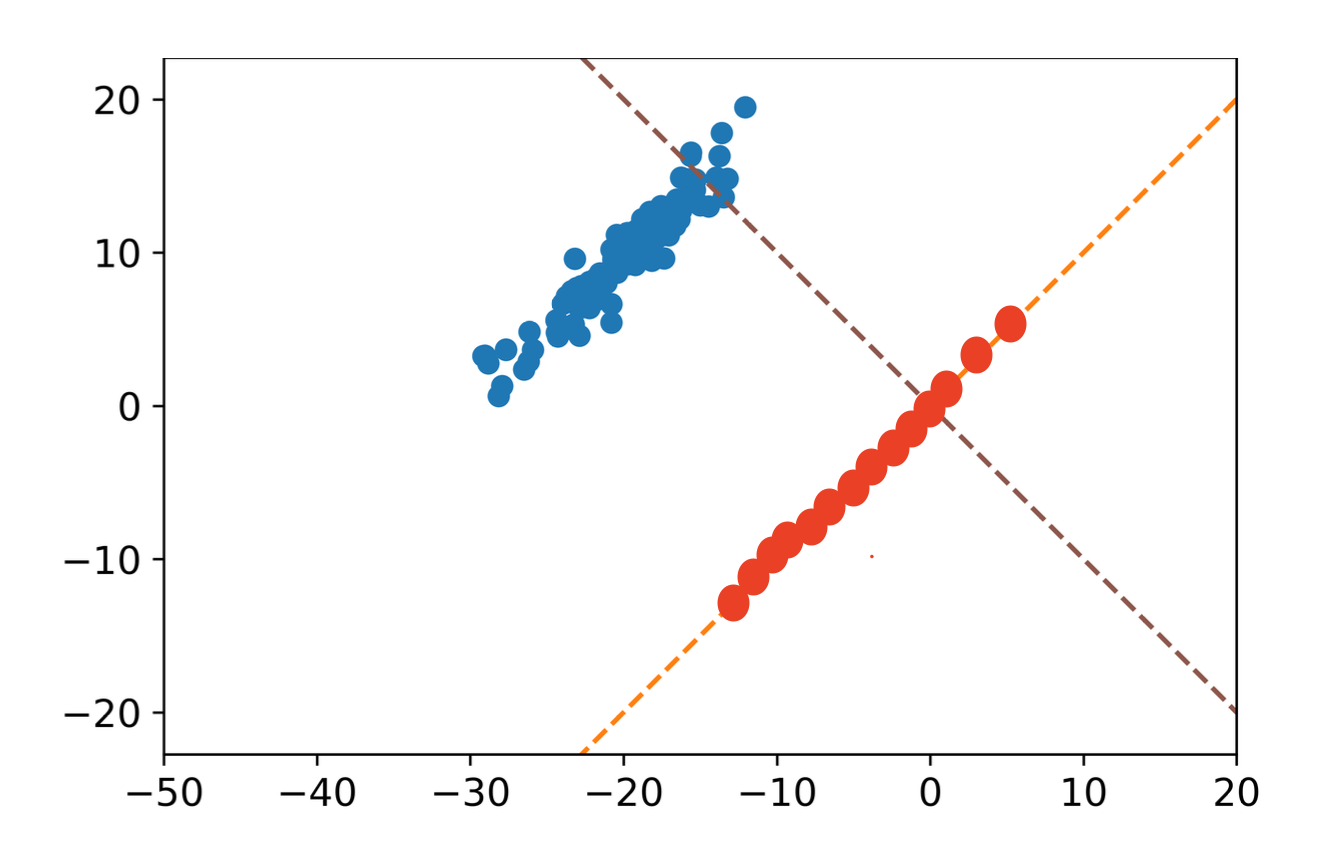
\includegraphics[width=0.7\textwidth]{proj.png}
    \caption{Projection of the data onto the first principal component}
    \label{fig:projection}
\end{figure}

\newpage
\section{Probabilistic PCA - A general latent space distribution}

\subsection*{a)}

Since 

\begin{align*}
    p(\bm{x} | \bm{z}) &= \mathcal{N}(\bm{W}\bm{z} + \bm{\mu}, \sigma^2 \bm{I}) \\
\end{align*}

Then we can say that:

\begin{align*}
    \epsilon_x &\sim \mathcal{N}(0, \sigma^2 \bm{I}) \\
\end{align*}

Now, since \( \bm{x} = \bm{W}\bm{z} + \bm{\mu} + \epsilon_x \) and $\bm{z} = \bm{m} + \epsilon_z$, we can rewrite the expression as:

\begin{align*}
    \bm{x} &= \bm{W}(\bm{m} + \epsilon_z) + \bm{\mu} + \epsilon_x \\
    &= \bm{W}\bm{m} + \bm{W}\epsilon_z + \bm{\mu} + \epsilon_x \\
\end{align*}

Now, since \( \bm{W}\epsilon_z \) is a linear transformation of a Gaussian random variable, it is also Gaussian.
Therefore, \( \bm{W}\epsilon_z \sim \mathcal{N}(0, \bm{W} \Sigma \bm{W}^T) \) (this will be shown in the next question).

With this, since the sum of two Gaussian random variables is also Gaussian, we have that:

\begin{align*}
    \bm{x} &\sim \mathcal{N}(\bm{W}\bm{m} + \bm{\mu}, \bm{W} \Sigma \bm{W}^T + \sigma^2 \bm{I}) \\
\end{align*}

Note: We can ignore the $\bm{W}(\bm{m} + \bm{\mu}$ because they are constants and do not affect the type of distribution of $\bm{x}$.

\subsection*{b)}

To find the expectation of the variable $\bm{x}$ by taking into account the linearity of the expectation operator, we have that:

\begin{align*}
    E[\bm{x}] &= E[\bm{W}\bm{m} + \bm{\mu} + \epsilon_x + \bm{W}\epsilon_z] \\
    &= E[\bm{W}\bm{m}] + E[\bm{\mu}] + E[\epsilon_x] + E[\bm{W}\epsilon_z] \\
    &= \bm{W}\bm{m} + \bm{\mu} + E[\epsilon_x] + W E[\epsilon_z] \\
    &= \bm{W}\bm{m} + \bm{\mu}
\end{align*}

This, because the expectancy of a constant is the constant itself in the case of $\bm{W}\bm{m}$ and $\bm{\mu}$, and the expectancy of a Gaussian random variable is the mean of the Gaussian distribution,
which is 0 in the case of $\epsilon_x$, since $\epsilon_x \sim \mathcal{N}(0, \sigma^2 \bm{I})$ and in the case of $\bm{W}\epsilon_z$, since $\epsilon_z \sim \mathcal{N}(0, \Sigma)$.

\subsection*{c)}

To find the covariance of the variable $x$, we have that:

\begin{align*}
    Cov[\bm{x}, \bm{x}] &= Var[\bm{x}] \\
    &= Var[\bm{W}\bm{m} + \bm{\mu} + \epsilon_x + \bm{W}\epsilon_z] \\
    &= Var[\bm{W}\bm{m}] + Var[\bm{\mu}] + Var[\epsilon_x] + Var[\bm{W}\epsilon_z] \\
    &= \bm{W} Var[m] \bm{W}^T + Var[\bm{\mu}] + Var[\epsilon_x] + \bm{W} Var[\epsilon_z] \bm{W}^T \\
    &= \bm{W} Var[m] \bm{W}^T + Var[\epsilon_x] + \bm{W} Var[\epsilon_z] \bm{W}^T \\
    &= \bm{W} Var[m] \bm{W}^T + \sigma^2 \bm{I} + \bm{W} \bm{\Sigma} \bm{W}^T \\
    &= \sigma^2 \bm{I} + \bm{W} \bm{\Sigma} \bm{W}^T \quad \text{since $Var[m] = Var[\bm{\mu}] = 0$ because they are constants} \\
    &= \sigma^2 \bm{I} + \bm{W} \bm{\Sigma} \bm{W}^T \quad \text{since $Var[\epsilon_x] = \sigma^2 \bm{I}$ and $Var[\epsilon_z] = \bm{\Sigma}$}
\end{align*}

This, because the covariance of a Gaussian random variable is the covariance matrix of the Gaussian distribution. 

\subsection*{d)}

To match the previous expression for the General Gaussian prior:

\begin{align*}
    \bm{x} &\sim \mathcal{N}(\bm{W}\bm{m} + \bm{\mu}, \bm{W} \bm{\Sigma} \bm{W}^T + \sigma^2 \bm{I}) \\
\end{align*}

In the form:

\begin{align*}
    \bm{x} &\sim \mathcal{N}(\tilde{\bm{\mu}}, \bm{\tilde{W}} \bm{\tilde{W}}^T + \sigma^2 \bm{I}) \\
\end{align*}

We have that:

\begin{align*}
    \tilde{\bm{\mu}} &= \bm{W}\bm{m} + \bm{\mu} \\
    \bm{\tilde{W}} &= \bm{W} \bm{\Sigma}^{1/2}
\end{align*}

The $\tilde{\bm{\mu}}$ is easy to check because it is the mean of the Gaussian distribution, and the $\bm{\tilde{W}}$ is the square root of the covariance matrix of the Gaussian distribution, since:

\begin{align*}
    \bm{W} \bm{\Sigma} \bm{W}^T + \sigma^2 \bm{I} &= \bm{W} \bm{\Sigma}^{1/2} \bm{\Sigma}^{1/2} \bm{W}^T + \sigma^2 \bm{I} \\
    &= \bm{W} \bm{\Sigma}^{1/2} {\bm{\Sigma}^{1/2}}^T \bm{W}^T + \sigma^2 \bm{I} \quad \text{since $\bm{\Sigma}$ is symmetric} \\
    &= (\bm{W} \bm{\Sigma}^{1/2}) (\bm{W} \bm{\Sigma}^{1/2})^T + \sigma^2 \bm{I}
\end{align*}

\section{Mixtures of Experts}

\subsection*{a)}

Considering that $z_n$ is one-hot encoded, then we assign 1 to the index corresponding to the expert that is responsible
for the data point $\bm{x_n}$, i.e., the one with the highest probability, and 0 to the other indices.
In resume, we need to find the index $k$ that maximizes the probability $p(z_n = k | \bm{x_n}, \Phi) = \pi_{nk}$.

This gives that:

\begin{align*}
    z_n = \underset{j}{\mathrm{argmax}} \pi_{nk}
    &= \begin{cases}
        1, & \text{if } k = \underset{j}{\mathrm{argmax}} \pi_{nj} = \underset{j}{\mathrm{argmax}} \frac{exp(\phi_j^T \bm{x_n})}{\sum_{l=1}^{K} exp(\bm{\phi_l}^T \bm{x_n})} \\
        0, & \text{otherwise}
    \end{cases}
\end{align*}

\subsection*{b)}

The likelihood of the data is given by:

\begin{align*}
    p(\bm{y} | \bm{X}, \bm{\Theta}, \bm{\Phi}) &= \prod_{n=1}^{N} p(\bm{y_n} | \bm{x_n}, \Theta, \Phi) \quad \text{assuming i.i.d.} \\
    &= \prod_{n=1}^{N} \sum_{k=1}^{K} p(\bm{y_n} | \bm{z_n} = k, \bm{x_n}, \Theta) p(\bm{z_n} = k | \bm{x_n}, \Phi) \quad \text{marginalizing $\bm{z_n}$ over experts} \\
    &= \prod_{n=1}^{N} \sum_{k=1}^{K} \pi_{nk} p(\bm{y_n} | \bm{z_n} = k, \bm{x_n}, \Theta) \\
\end{align*}

Which, if we expand the terms, gives:

\begin{align*}
    p(\bm{y} | \bm{X}, \bm{\Theta}, \bm{\Phi}) &= \prod_{n=1}^{N} \sum_{k=1}^{K} \frac{\exp(\bm{\phi_k}^T \bm{x_n})}{\sum_{l=1}^{K} \exp(\bm{\phi_l}^T \bm{x_n})} \exp(\bm{\theta_k}^T \bm{x_n}) \exp(-\exp(\bm{\theta_k}^T \bm{x_n}) \bm{y_n}) \\
    &= \prod_{n=1}^{N} \sum_{k=1}^{K} \frac{\exp(\bm{\phi_k}^T \bm{x_n})}{\sum_{l=1}^{K} \exp(\bm{\phi_l}^T \bm{x_n})} \exp(\bm{\theta_k}^T \bm{x_n} -\exp(\bm{\theta_k}^T \bm{x_n}) \bm{y_n}) \\
\end{align*}

The log-likelihood, without the expanding terms, is given by:

\begin{align*}
    \log p(\bm{y} | \bm{X}, \bm{\Theta}, \bm{\Phi}) &= \sum_{n=1}^{N} \log \sum_{k=1}^{K} \pi_{nk} p(\bm{y_n} | \bm{z_n} = k, \bm{x_n}, \Theta) \\
\end{align*}

Expanding the terms, we have:

\begin{align*}
    \log p(\bm{y} | \bm{X}, \bm{\Theta}, \bm{\Phi}) &= \sum_{n=1}^{N} \log \sum_{k=1}^{K} \frac{\exp(\bm{\phi_k}^T \bm{x_n})}{\sum_{l=1}^{K} \exp(\bm{\phi_l}^T \bm{x_n})} \exp(\bm{\theta_k}^T \bm{x_n} -\exp(\bm{\theta_k}^T \bm{x_n}) \bm{y_n}) \\
\end{align*}

\subsection*{c)}

The responsability of the expert $i$ for the data point $\bm{x_n}$ is given by:

\begin{align*}
    r_{ni} &= p(z_{ni} = 1 | \bm{x_n}, \Theta, \Phi) \\
    &= \frac{p(\bm{y_n} | \bm{x_n}, z_{ni} = 1, \Theta) p(z_{ni} = 1 | \bm{x_n}, \Phi)}{p(\bm{y_n} | \bm{x_n}, \Theta, \Phi)} \\
    &= \frac{p(\bm{y_n} | z_{ni} = 1, \bm{x_n}, \Theta) p(z_{ni} = 1 | \bm{x_n}, \Phi)}{\sum_{j=1}^{K} p(\bm{y_n} | z_{nj} = 1, \bm{x_n}, \Theta) p(z_{nj} = 1 | \bm{x_n}, \Phi)} \\
    &= \frac{\pi_{nk} p(\bm{y_n} | z_{ni} = 1, \bm{x_n}, \Theta)}{\sum_{j=1}^{K} \pi_{nj} p(\bm{y_n} | z_{nj} = 1, \bm{x_n}, \Theta)} \\
\end{align*}

By expanding the terms, we have:

\begin{align*}
    r_{ni} &= \frac{\frac{\exp(\bm{\phi_i}^T \bm{x_n})}{\sum_{l=1}^{K} \exp(\bm{\phi_l}^T \bm{x_n})} \exp(\bm{\theta_i}^T \bm{x_n} -\exp(\bm{\theta_i}^T \bm{x_n}) \bm{y_n})}{\sum_{j=1}^{K} \frac{\exp(\phi_j^T \bm{x_n})}{\sum_{l=1}^{K} \exp(\bm{\phi_l}^T \bm{x_n})} \exp(\theta_j^T \bm{x_n} -\exp(\theta_j^T \bm{x_n}) \bm{y_n})} \\
\end{align*}

Which can be simplified to:

\begin{align*}
    r_{ni} &= \frac{\exp(\bm{\phi_i}^T \bm{x_n}) \exp(\bm{\theta_i}^T \bm{x_n} -\exp(\bm{\theta_i}^T \bm{x_n}) \bm{y_n})}{\sum_{j=1}^{K} \exp(\phi_j^T \bm{x_n}) \exp(\theta_j^T \bm{x_n} -\exp(\theta_j^T \bm{x_n}) \bm{y_n})} \\
\end{align*}

\subsection*{d)}

As shown before, the likelihood is given by:

\begin{align*}
    p(\bm{y} | \bm{X}, \bm{\Theta}, \bm{\Phi}) &= \prod_{n=1}^{N} \sum_{k=1}^{K} p(\bm{z_n} = k | \bm{x_n}, \Phi) p(\bm{y_n} | \bm{z_n} = k, \bm{x_n}, \Theta) \\
\end{align*}

By taking the hint into account to derivate the log-likelihood, we have that:

\begin{align*}
    \frac{\partial \log p(\bm{y} | \bm{X}, \bm{\Theta}, \bm{\Phi})}{\partial \bm{\theta_i}} &= \frac{\partial}{\partial \bm{\theta_i}} \sum_{n=1}^{N} \log \sum_{k=1}^{K} p(\bm{z_n} = k | \bm{x_n}, \Phi) p(\bm{y_n} | \bm{z_n} = k, \bm{x_n}, \bm{\theta_k}) \\
    &= \sum_{n=1}^{N} \frac{\partial}{\partial \bm{\theta_i}} \log \sum_{k=1}^{K} p(\bm{z_n} = k | \bm{x_n}, \Phi) p(\bm{y_n} | \bm{z_n} = k, \bm{x_n}, \bm{\theta_k}) \\
    &= \sum_{n=1}^{N} \frac{1}{\sum_{k=1}^{K} p(\bm{z_n} = k | \bm{x_n}, \Phi) p(\bm{y_n} | \bm{z_n} = k, \bm{x_n}, \bm{\theta_k})} \frac{\partial}{\partial \bm{\theta_i}} \sum_{k=1}^{K} p(\bm{z_n} = k | \bm{x_n}, \Phi) p(\bm{y_n} | \bm{z_n} = k, \bm{x_n}, \bm{\theta_k}) \\
    &= \sum_{n=1}^{N} \frac{1}{\sum_{k=1}^{K} p(\bm{z_n} = k | \bm{x_n}, \Phi) p(\bm{y_n} | \bm{z_n} = k, \bm{x_n}, \bm{\theta_k})} \sum_{k=1}^{K} \frac{\partial}{\partial \bm{\theta_i}} p(\bm{z_n} = k | \bm{x_n}, \Phi) p(\bm{y_n} | \bm{z_n} = k, \bm{x_n}, \bm{\theta_k}) \\
\end{align*}
Since, $p(\bm{z_n} = k | \bm{x_n}, \Phi)$ does not depend on $\bm{\theta_i}$, we have that:

\begin{align*}
    \frac{\partial \log p(\bm{y} | \bm{X}, \bm{\Theta}, \bm{\Phi})}{\partial \bm{\theta_i}} &= \sum_{n=1}^{N} \frac{1}{\sum_{k=1}^{K} p(\bm{z_n} = k | \bm{x_n}, \Phi) p(\bm{y_n} | \bm{z_n} = k, \bm{x_n}, \bm{\theta_k})} \sum_{k=1}^{K} p(\bm{z_n} = k | \bm{x_n}, \Phi) \frac{\partial}{\partial \bm{\theta_i}} p(\bm{y_n} | \bm{z_n} = k, \bm{x_n}, \bm{\theta_k}) \\
\end{align*}

Now, taking the derivative in respect of $\bm{\phi_i}$:

\begin{align*}
    \frac{\partial \log p(\bm{y} | \bm{X}, \bm{\Theta}, \bm{\Phi})}{\partial \bm{\phi_i}} &= \frac{\partial}{\partial \bm{\phi_i}} \sum_{n=1}^{N} \log \sum_{k=1}^{K} p(\bm{z_n} = k | \bm{x_n}, \Phi) p(\bm{y_n} | \bm{z_n} = k, \bm{x_n}, \bm{\theta_k}) \\
    &= \sum_{n=1}^{N} \frac{\partial}{\partial \bm{\phi_i}} \log \sum_{k=1}^{K} p(\bm{z_n} = k | \bm{x_n}, \Phi) p(\bm{y_n} | \bm{z_n} = k, \bm{x_n}, \bm{\theta_k}) \\
    &= \sum_{n=1}^{N} \frac{1}{\sum_{k=1}^{K} p(\bm{z_n} = k | \bm{x_n}, \Phi) p(\bm{y_n} | \bm{z_n} = k, \bm{x_n}, \bm{\theta_k})} \frac{\partial}{\partial \bm{\phi_i}} \sum_{k=1}^{K} p(\bm{z_n} = k | \bm{x_n}, \Phi) p(\bm{y_n} | \bm{z_n} = k, \bm{x_n}, \bm{\theta_k}) \\
    &= \sum_{n=1}^{N} \frac{1}{\sum_{k=1}^{K} p(\bm{z_n} = k | \bm{x_n}, \Phi) p(\bm{y_n} | \bm{z_n} = k, \bm{x_n}, \bm{\theta_k})} \sum_{k=1}^{K} \frac{\partial}{\partial \bm{\phi_i}} p(\bm{z_n} = k | \bm{x_n}, \Phi) p(\bm{y_n} | \bm{z_n} = k, \bm{x_n}, \bm{\theta_k}) \\
\end{align*}

Now, since $p(\bm{y_n} | \bm{z_n} = k, \bm{x_n}, \bm{\theta_k})$ does not depend on $\bm{\phi_i}$, we have that:

\begin{align*}
    \frac{\partial \log p(\bm{y} | \bm{X}, \bm{\Theta}, \bm{\Phi})}{\partial \bm{\phi_i}} &= \sum_{n=1}^{N} \frac{1}{\sum_{k=1}^{K} p(\bm{z_n} = k | \bm{x_n}, \Phi) p(\bm{y_n} | \bm{z_n} = k, \bm{x_n}, \Theta)} \sum_{k=1}^{K} p(\bm{y_n} | \bm{z_n} = k, \bm{x_n}, \bm{\theta_k}) \frac{\partial}{\partial \bm{\phi_i}} p(\bm{z_n} = k | \bm{x_n}, \Phi) \\
\end{align*}

\textbf{Note:} The responsabilities only appear when taking the explicitly derivation of the probabilities,
since it will depende on the values of the probabilities. This is be shown in the next question.


\newpage
\subsection*{e)}

Now, inserting the explicit expressions for the probabilities, we have that:

\begin{align*}
    \frac{\partial \log p(\bm{y} | \bm{X}, \bm{\Theta}, \bm{\Phi})}{\partial \bm{\theta_i}} &= \sum_{n=1}^{N} \frac{1}{\sum_{k=1}^{K} \pi_{nk} p(\bm{y_n} | \bm{z_n} = k, \bm{x_n}, \bm{\Theta})} \frac{\partial}{\partial \bm{\theta_i}} \sum_{k=1}^{K} p(\bm{z_n} = k | \bm{x_n}, \Phi) p(\bm{y_n} | \bm{z_n} = k, \bm{x_n}, \bm{\theta_k}) \\
    &= \sum_{n=1}^{N} \frac{1}{\sum_{k=1}^{K} \pi_{nk} p(\bm{y_n} | \bm{z_n} = k, \bm{x_n}, \bm{\Theta})} \frac{\partial}{\partial \bm{\theta_i}} \sum_{k=1}^{K} \pi_{nk} p(\bm{y_n} | \bm{z_n} = k, \bm{x_n}, \Theta) \\
\end{align*}

Since $\pi_{nk}$ does not depend on $\bm{\theta_i}$, we have that:

\begin{align*}
    \frac{\partial \log p(\bm{y} | \bm{X}, \bm{\Theta}, \bm{\Phi})}{\partial \bm{\theta_i}} &= \sum_{n=1}^{N} \frac{1}{\sum_{k=1}^{K} \pi_{nk} p(\bm{y_n} | \bm{z_n} = k, \bm{x_n}, \bm{\Theta})} \sum_{k=1}^{K} \pi_{nk} \frac{\partial}{\partial \bm{\theta_i}} p(\bm{y_n} | \bm{z_n} = k, \bm{x_n}, \Theta) \\
    &= \sum_{n=1}^{N} \frac{\pi_{nk}}{\sum_{k=1}^{K} \pi_{nk} p(\bm{y_n} | \bm{z_n} = k, \bm{x_n}, \bm{\Theta})} \sum_{k=1}^{K} \frac{\partial}{\partial \bm{\theta_i}} \left(\lambda \exp(-\lambda \bm{y_n}) \right) \\
    &= \sum_{n=1}^{N} \frac{\pi_{nk}}{\sum_{k=1}^{K} \pi_{nk} p(\bm{y_n} | \bm{z_n} = k, \bm{x_n}, \bm{\Theta})} \sum_{k=1}^{K} \frac{\partial}{\partial \lambda} \left(\lambda \exp(-\lambda \bm{y_n}) \right) \frac{\partial \lambda}{\partial \bm{\theta_i}} \quad \text{by the chain rule} \\
    &= \sum_{n=1}^{N} \frac{\pi_{nk}}{\sum_{k=1}^{K} \pi_{nk} p(\bm{y_n} | \bm{z_n} = k, \bm{x_n}, \bm{\Theta})} \sum_{k=1}^{K} (\exp(-\lambda \bm{y_n}) - \lambda \bm{y_n} \exp(-\lambda \bm{y_n})) \frac{\partial \lambda}{\partial \bm{\theta_i}} \\
    &= \sum_{n=1}^{N} \frac{\pi_{nk}}{\sum_{k=1}^{K} \pi_{nk} p(\bm{y_n} | \bm{z_n} = k, \bm{x_n}, \bm{\Theta})} \sum_{k=1}^{K} (\exp(-\lambda \bm{y_n}) - \lambda \bm{y_n} \exp(-\lambda \bm{y_n})) \frac{\partial}{\partial \bm{\theta_i}} \exp(\bm{\theta_k}^T \bm{x_n}) \\
    &= \sum_{n=1}^{N} \frac{\pi_{nk}}{\sum_{k=1}^{K} \pi_{nk} p(\bm{y_n} | \bm{z_n} = k, \bm{x_n}, \bm{\Theta})} \sum_{k=1}^{K} (\exp(-\lambda \bm{y_n}) - \lambda \bm{y_n} \exp(-\lambda \bm{y_n})) \exp(\bm{\theta_k}^T \bm{x_n}) \bm{x_n}^T \delta_{ik} \\
    &= \sum_{n=1}^{N} \frac{\pi_{ni}}{\sum_{k=1}^{K} \pi_{nk} p(\bm{y_n} | \bm{z_n} = k, \bm{x_n}, \bm{\Theta})} (\exp(-\lambda \bm{y_n}) - \lambda \bm{y_n} \exp(-\lambda \bm{y_n})) \exp(\bm{\theta_i}^T \bm{x_n}) \bm{x_n}^T \\
    &= \sum_{n=1}^{N} \frac{\pi_{ni}}{\sum_{k=1}^{K} \pi_{nk} p(\bm{y_n} | \bm{z_n} = k, \bm{x_n}, \bm{\Theta})} \lambda \exp(-\lambda \bm{y_n}) (\mathds{1} - \lambda \bm{y_n}) \bm{x_n}^T \\
    &= \sum_{n=1}^{N} \frac{\pi_{ni} p(\bm{y_n} | \bm{z_n} = i, \bm{x_n}, \bm{\theta_i})}{\sum_{k=1}^{K} \pi_{nk} p(\bm{y_n} | \bm{z_n} = k, \bm{x_n}, \bm{\Theta})} (\mathds{1} - \lambda \bm{y_n}) \bm{x_n}^T \quad \text{since $p(\bm{y_n} | \bm{z_n} = i, \bm{x_n}, \bm{\theta_i}) = \lambda \exp(-\lambda \bm{y_n})$} \\
    &= \sum_{n=1}^{N} r_{ni} \bm{x_n}^T (\mathds{1} - \lambda \bm{y_n}) 
\end{align*}

Now, for $\bm{\phi_i}$:

\begin{align*}
    \frac{\partial \log p(\bm{y} | \bm{X}, \bm{\Theta}, \bm{\Phi})}{\partial \bm{\phi_i}} &= \sum_{n=1}^{N} \frac{1}{\sum_{k=1}^{K} \pi_{nk} p(\bm{y_n} | \bm{z_n} = k, \bm{x_n}, \phi)} \frac{\partial}{\partial \bm{\phi_i}} \sum_{k=1}^{K} p(\bm{z_n} = k | \bm{x_n}, \Phi) p(\bm{y_n} | \bm{z_n} = k, \bm{x_n}, \bm{\phi_k}) \\
    &= \sum_{n=1}^{N} \frac{1}{\sum_{k=1}^{K} \pi_{nk} p(\bm{y_n} | \bm{z_n} = k, \bm{x_n}, \Theta)} \frac{\partial}{\partial \bm{\phi_i}} \sum_{k=1}^{K} \pi_{nk} p(\bm{y_n} | \bm{z_n} = k, \bm{x_n}, \Theta) \\
    &= \sum_{n=1}^{N} \frac{1}{\sum_{k=1}^{K} \pi_{nk} p(\bm{y_n} | \bm{z_n} = k, \bm{x_n}, \Theta)}  \sum_{k=1}^{K} \frac{\partial}{\partial \bm{\phi_i}} \pi_{nk} p(\bm{y_n} | \bm{z_n} = k, \bm{x_n}, \Theta) \\
    &= \sum_{n=1}^{N} \frac{1}{\sum_{k=1}^{K} \pi_{nk} p(\bm{y_n} | \bm{z_n} = k, \bm{x_n}, \Theta)}  \sum_{k=1}^{K} p(\bm{y_n} | \bm{z_n} = k, \bm{x_n}, \Theta) \frac{\partial}{\partial \bm{\phi_i}} \pi_{nk}  \\
    &= \sum_{n=1}^{N} \frac{1}{\sum_{k=1}^{K} \pi_{nk} p(\bm{y_n} | \bm{z_n} = k, \bm{x_n}, \Theta)}  \sum_{k=1}^{K} p(\bm{y_n} | \bm{z_n} = k, \bm{x_n}, \Theta) \frac{\partial}{\partial \bm{\phi_i}} \frac{\exp(\bm{\phi_k}^T \bm{x_n})}{\sum_{l=1}^{K} \exp(\bm{\phi_l}^T \bm{x_n})}  \\
    &= \sum_{n=1}^{N} \frac{p(\bm{y_n} | z_n = k, \bm{x_n}, \Theta) \pi_{ni} (1 - \pi_{ni}) \bm{x_n}^T - \sum_{k \neq i}^{K} p(\bm{y_n} | z_n = k, \bm{x_n}, \Theta) \pi_{nk} \pi_{ni} \bm{x_n}^T}{\sum_{k=1}^{K} \pi_{nk} p(\bm{y_n} | z_n = k, \bm{x_n}, \Theta)}   \\
    &= \sum_{n=1}^{N} \left[r_{ni} (1 - \pi_{ni}) \bm{x_n}^T - \sum_{k \neq i}^{K} r_{nk} \pi_{ni} \bm{x_n}^T \right] \\
    &= \sum_{n=1}^{N} \left[r_{ni} (1 - \pi_{ni}) \bm{x_n}^T - \pi_{ni} \bm{x_n}^T \sum_{k \neq i}^{K} r_{nk}\right]  \\
    &= \sum_{n=1}^{N} \left[r_{ni} (1 - \pi_{ni}) \bm{x_n}^T - \pi_{ni} \bm{x_n}^T (1 - r_{ni})\right] \quad \text{since $\sum_{k=1}^{K} r_{nk} = 1 \rightarrow \sum_{k \neq i}^{K} r_{nk} = 1 - r_{ni}$} \\
    &= \sum_{n=1}^{N} \left[r_{ni} - \pi_{ni}\right] \bm{x_n}^T
\end{align*}

\newpage
\subsection*{f)}

Writing down an iterative algorithm that maximizes the log-probability by jointly optimizing the parameters $\Theta$ and $\Phi$:


\begin{algorithm}
    \caption{Joint optimization of \( \Theta \) and \( \Phi \) in Mixtures of Experts}
    \begin{algorithmic}
        \State \textbf{Input:} Data \( X \), labels \( Y \), parameters \( \Theta \), \( \Phi \), learning rate \( \alpha \), tolerance \( \epsilon \), maximum iterations
        \State \textbf{Output:} Updated parameters \( \Theta \), \( \Phi \)
        \State Initialize parameters \( \Theta \) and \( \Phi \)
        
        \While{not converged}
            \State \textbf{E-step:} Compute responsibilities \( r_{nk} \):
            \[
            r_{nk} = \frac{p(\bm{y_n} | \bm{x_n}, \bm{\theta_k}) \, \pi_{nk}}{\sum_{j=1}^{K} p(\bm{y_n} | \bm{x_n}, \bm{\theta}_j) \, \pi_{nj}}
            \]
            where \( \pi_{nk} = p(\bm{z_n} = k | \bm{x_n}, \Phi) = \frac{\exp(\bm{\phi_k}^T \bm{x_n})}{\sum_{j=1}^{K} \exp(\phi_j^T \bm{x_n})} \)
            
            \State \textbf{M-step:} Update \( \Theta \) and \( \Phi \) using the gradients:
            \[
            \theta_i^T \leftarrow \theta_i^T + \alpha \sum_{n=1}^{N} r_{ni} \bm{x_n}^T \left( \mathds{1} - \lambda \bm{y_n} \right) 
            \]
            \[
            \phi_i^T \leftarrow \phi_i^T + \alpha \sum_{n=1}^{N} \left[ r_{ni} - \pi_{ni} \right] \bm{x_n}^T
            \]
            \State \textbf{Check for convergence:} 
            \State \quad Compute the change in log-likelihood:
            \[
            \Delta \mathcal{L} = \left| \mathcal{L}^{(t+1)} - \mathcal{L}^{(t)} \right|
            \]
            \If{ \( \Delta \mathcal{L} < \epsilon \) \textbf{or} maximum iterations reached}
                \State \textbf{Terminate:} The algorithm has converged when the log-likelihood improvement is smaller than a predefined threshold \( \epsilon \), indicating that further updates provide negligible improvement.
                \State \quad \textbf{Return} optimized parameters \( \Theta \) and \( \Phi \).
            \Else
                \State \quad Continue to the next iteration by updating \( t \leftarrow t + 1 \).
            \EndIf
        \EndWhile
    \end{algorithmic}
\end{algorithm}


\newpage
\subsection*{g)}

If instead of having a single expert, we have multiple experts, then the final prediction $\bm{\hat{y}}$ is given by
the weighted sum of the predictions of each expert, where the weights are given by the responsibilities $r_{nk}$:

\begin{align*}
    \bm{\hat{y}} &= \sum_{k=1}^{K} r_{nk} \bm{\hat{y}}_{nk} \\
\end{align*}

This $\bm{\hat{y}}_{nk}$ is the prediction of the expert $k$ for the data point $\bm{x_n}$, which can be
sampled from the distribution of expert $k$.



\clearpage

\appendix


\newpage
\printbibliography

\end{document}

